\documentclass[pre,amsmath,preprintnumbers,10pt,article,notitlepage,twocolumn]{revtex4-1}
\usepackage{amsbsy}
\usepackage{graphicx,stmaryrd,wasysym}
\usepackage{color}
\usepackage{subfigure}
\usepackage{physics}
\usepackage{soul}
\usepackage{color}
\usepackage{bm}
\usepackage[normalem]{ulem}
\usepackage{amsmath}

%\newcommand{\Tr}{\text{Tr}}
\newcommand{\Ai}{\text{Ai}}
\newcommand{\Bi}{\text{Bi}}
\newcommand{\Real}{\text{Re}}
\newcommand{\Imag}{\text{Im}}

\usepackage{verbatim}
\usepackage{natbib}
\bibliographystyle{apsrev4-1}
\begin{document}
\title{How does dissipation constrain fluctuations beyond equilibrium? Consequences for diffusion and structure of driven fluids}
\author{Laura Tociu$^{1,3}$, Etienne Fodor$^{2}$, Suriyanarayanan Vaikuntanathan$^{1,3}$} 
\affiliation{$^1$The James Franck Institute, The University of Chicago, Chicago, IL,USA,}
\affiliation{$^2$ DAMTP, University of Cambridge,Cambridge,UK,}
\affiliation{$^3$ Department of Chemistry, The University of Chicago, Chicago, IL, USA}
\begin{abstract}
Nonequilibrium systems are generally regarded as an opportunity to create any kind of dynamics and structure by waving down the constraints of equilibrium. Yet, the emergent collective effects, when driven by a net flux of energy, are actually also constrained out-of-equilibrium. We first put forward a generic relation between the spontaneous fluctuations, quantified by the diffusion coefficient, and the amount of work produced by an external drive, related to energy dissipation. Second, we demonstrate how the hierarchy between density correlations, which enforces the fluid structure, is now affected by sustained energy dissipation. Using perturbation methods, we illustrate our findings for a fluid of colloidal particles driven by a periodic forcing.
\end{abstract}
\maketitle 

\section{Introduction}


Non-equilibrium forces can drive specific and novel pathways to modulate self-assembly and organization in materials. The close connection between energy dissipation and organization is especially apparent in living systems~\cite{Battle604}. This is particularly well illustrated by the remarkable properties of the flagella motors in E. Coli~\cite{Lele2013,Lan2012,Tu2017}. These motors exhibit unique phenomenology such as ultrasensitive response, adaptation, and motor restructuring as a function of applied torque. This phenomenology cannot be explained using classical equilibrium statistical mechanics models~\cite{Lan2012,Tu2017}. In fact, recent experimental work has shown that non-equilibrium forces are responsible for the hierarchical self-organization of the motor and the abovementioned phenomenology~\cite{Wang2017,Tu2017}. In vitro studies of the cellular cytoskeleton and in vivo studies of model actin and microtubule systems driven by molecular motors have also shown how non-equilibrium forces can be used to achieve a variety of functionality not allowed at equilibrium~\cite{Decamp2015,Ramaswamy2010,Sanchez2012}. Such studies have for instance demonstrated how non-equilibrium materials can sense forces robustly and adapt to their surroundings~\cite{Decamp2015}. 

In order to understand how non-equilibrium forces can be used to generate such properties in materials, it important to theoretically and computationally understand how material properties and responses are modified by non-equilibrium flows of energy. However, while the behavior and characteristics of equilibrium systems - where no energy is dissipated - are well known, progress in the area of non-equilibrium control has been hampered by a lack of general principles that characterize non-equilibrium steady states and fluctuations about them~\cite{Takatori2015,Fodor2016,Cates2015,Solon2015a,Nguyen2016,Murugan2017,Nguyen2018}. 


In a recent work~\cite{delJunco2018}, we reported on the structure, transport and phase properties of a model system consisting of a mixture of driven and undriven Brownian particles~\cite{Han2016}. We found that the energy injected into the system by the driving forces, which we called $w$ (\textit{work}) Eq.~\ref{eq:wdef}, led to a renormalization of force fluctuations - changing the environment felt by the particles - and modified the diffusion coefficient of the particles in the system. In this previous work, we found that Gaussian density fluctuations~\cite{Chandler1993}, which we identified in the liquid, helped give insight into the observed behavior of the various quantities we examined and their scaling with the driving forces.

In this paper we wish to explore more precisely and quantitatively how energy flows modify properties of driven liquids. To this end we consider a theoretical model of a driven tracer in a Gaussian fluctuating field~\cite{Chandler1993,Dean1996,Kruger2017,Demery2014}, accompanied by numerical simulations of a system with Brownian particles, a small fraction of which are driven in circular radii. The radius is determined by the amplitude $Pe$ and time period $\tau\equiv 2 \pi/\omega$ of the driving force. We solve the theoretical model using a perturbation theory and extract expressions for the diffusion constant, work ($\langle w \rangle$) done by the external fields on the tracer particles in the limit of high and low driving frequencies, $\omega$. In the limit of high driving frequencies, our perturbation theory shows that the increase in the diffusion constant of the tracer particle and the rate at which work is done on the system, $\langle {\dot w} \rangle$, both scale like $Pe^2/\omega^2$. In the low frequency limit, our calculations show that whenever $\langle w \rangle$ scales like $Pe^2$, the increase in the diffusion constant also exhibits the same scaling. These theoretical results demonstrate the interplay between energy consumption and transport in this non-equilibrium system~\cite{delJunco2018}. 

Next, we obtain expressions for energy fluxes within this perturbation theory and show how $w$ renormalizes the environment around a driven particle. The relationship we find between work, force fluctuations, and energy change of the bath can be seen as yet another form of the Harada-Sasa relation, which relates energy dissipation to the breakdown of the fluctuation dissipation relation~\cite{Harada2005, Harada2006}. Using this connection as a basis, we explore how the pair correlation function between the tracer particle and the environment are modified due to the non-equilibrium driving. 

Finally, motivated by these connections between work, transport, and structure, we construct biased ensembles in which we bias the probability of sampling trajectories~\cite{Chetrite2013,Jack2010} according to the amount of work being done on specific interactions. In qualitative agreement with the findings from the theoretical perturbation treatment analysis, we find that introducing such a bias on energy flows results in a renormalization of interactions between particles. Together, our results show how keeping track of simple scalar quantities such as energy fluxes or $\langle w\rangle$ can help constrain the material and transport properties of systems far from equilibrium. 

%To further study the effect of $w$ on the environment around the tracer, we compute the pair correlation function from simulation and explore its scaling with the driving forces as well. Going beyond the perturbative limit, we use a Kirkwood approximation to argue how $w$ can modify the pair correlation function.


\section{Methods}

\subsection{Theoretical Model}

The goal of our model is to resemble a tracer moving through a liquid exhibiting Gaussian density fluctuations~\cite{Chandler1993}. To accomplish this, we start with the general form of a Hamiltonian for a Gaussian density field interacting with a tracer whose position is determined by ${\bf r}_0(t)$:

\begin{equation}
\begin{split}
H(t) =& \dfrac{K_BT}{2} \int d{\bf r} \int d {\bf r}' \delta \rho ({\bf r}, t) \chi^{-1}({\bf r} - {\bf r}') \delta \rho ({\bf r}', t) + \\
&\int d{\bf r} V({\bf r} - {\bf r}_0(t))\delta \rho({\bf r}, t)
\end{split}
\end{equation}
where $\delta \rho({\bf r},t ) = \rho({\bf r}, t) - \rho_0 $ and $\rho_0$ is the density of the liquid. The covariance  is $\chi({\bf r}-{\bf r}')= \langle \delta \rho({\bf r}) \delta \rho ({\bf r}') \rangle=  \rho_0 \delta({\bf r} - {\bf r}') +\rho_0^2 g({\bf r}-{\bf r}')$, and $g({\bf r}-{\bf r}')$ is the two point correlation function. 
\\

% Note:  We imagine $\chi^{-1}({\bf r}-{\bf r'})$ to be scaled by the inverse of the square of the integration volume element, so as the double integral above is unitless.
%\\

The equation of motion of the density field can then be written as: 
\begin{equation}
\begin{split}
\frac{\partial \delta \rho({\bf r}, t)}{\partial t} =& - \dfrac{ K_BT}{\gamma_G} \nabla^2 \left[ \int  d{\bf r}' \chi^{-1} ({\bf r}-{\bf r}') \delta \rho({\bf r}', t)\right]  \\ &- \dfrac{ K_BT}{\gamma_G} \nabla^2 V({\bf r}-{\bf r}_0(t)) + \nabla \cdot \eta({\bf r},t)
\end{split}
\label{eq:EvolutionField}
\end{equation}
The noise is multiplicative, obeying $\langle \eta({\bf r}, t) \cdot \eta({\bf r}', t') \rangle = 2D_G \delta({\bf r} - {\bf r}')\delta(t-t')$, and the parameters $\gamma_G$ and $D_G$ are course-grained damping and diffusion coefficients.


% Note:  In the above, if we define a timescale $t_0 = r_0^2/D_0$, we get the following units for the two parameters: $\gamma_G \propto \frac{K_BT V t_0}{L^2}$, and $D_G \propto  \frac{\rho_0^2L^2}{t_0}$.  Thus, the fluctuation dissipation theorem would yield $D_G \gamma_G \propto K_BT V \rho_0^2$.

In Fourier space, Eq.~\ref{eq:EvolutionField} becomes:

\begin{equation}
\begin{split}
\frac{\partial \delta \rho({\bf q},t)}{\partial t} & = -\dfrac{1}{\gamma_G}\left[ K_BT |{\bf q}|^2 \chi^{-1}({\bf q}) \delta \rho({\bf q}) \right] \\ &-\dfrac{1}{\gamma_G}\left[ |{\bf q}|^2 V({\bf q}) e^{-i {\bf q} \cdot {\bf r}_0(t)} \right] + i{\bf q} \cdot \eta({\bf q},t)
\end{split}
\label{eq:FourierEvolutionField}
\end{equation}
where $\langle \eta({\bf q}, s) \cdot \eta({\bf q}', s')  \rangle = 2D_G \delta({\bf q} + {\bf q}') \delta(s-s')$.

%Note:  If the interparticle potential were zero, Eq. \ref{eq:FourierEvolutionField} could be solved yielding a probability distribution $P(\delta \rho({\bf q})) = e^{-\tfrac{K_BT \chi^{-1}({\bf q}) \delta \rho({\bf q})^2}{D_G \gamma_G}}$, which would have the right dimensions in the exponent, as expected.

The complementary equation of motion for an undriven tracer is:

\begin{equation}
\begin{split}
\dfrac{d{\bf r}_0(t)}{d t} & = -\dfrac{1}{\gamma} \int  d{\bf q} i {\bf q} V(-{\bf q})e^{i{\bf q} \cdot {\bf r}_0(t)} \delta \rho({\bf q}, t) +  \eta_0(t)\\
&\equiv \frac{1}{\gamma} {\bf F}(t) + \eta_0(t) 
\end{split}
\label{eq:EvolutionTracer}
\end{equation}
where  ${\bf F}(t)$ is the conservative force on the tagged particle from the medium, $\eta_0(t)$ is white noise of zero mean and variance $2D_0$, and $2D_0 ={K_BT}/{\gamma}$. The tracer is driven out of equilibrium by modifying Eq.~\ref{eq:EvolutionTracer} with an extra driving force 
\begin{align}
&{\bf F}_{\rm d} =A(\sin\theta \hat e_x+\cos\theta\hat e_y) \label{eq:FexEq} \\
&\theta=2\pi t/\tau. \label{eq:theta}
\end{align}
where A is an amplitude with units of force. The strength of the driving forces is expressed in terms of the Peclet number (ratio of advective to diffusive velocity), which we define as $Pe = \frac{A/\gamma}{D_0/r_0}$~\cite{delJunco2018,Han2016}. Thus, a single active particle will draw a circle in the 2D plane. In the following, we use the notation ${\bf F}_{\rm d}(t) \equiv Pe {\bf v} (t)$ to denote the external force. 

Eq.~\ref{eq:FourierEvolutionField} can be exactly solved if the tracer trajectory, ${\bf r}_0(t)$, is known. Specifically, by labeling $\chi^{-1}({\bf q}) = K({\bf q})$, the restoring force for density fluctuations, we get:

\begin{equation}
\begin{split}
\delta\rho({\bf q},t)=
&\int\limits_{-\infty}^t ds  e^{-\frac{K_BT}{\gamma_G}|{\bf q}|^2 K({\bf q})(t-s)}\left[-|{\bf q}|^2 \dfrac{V({\bf q})}{\gamma_G} e^{-i {\bf q}\cdot {\bf r}_0(s)}\right] \\ & +\int\limits_{-\infty}^t ds \left[ i{\bf q} \cdot \eta({\bf q},s)\right] 
\end{split}
\label{eq:SolutionFourierEvolution}
\end{equation}

Putting everything together, the full conservative force acting on the tracer in this formalism is:

\begin{equation}
\begin{split}
{\bf F}(t) &= -\int d{\bf q} i{\bf q} V(-{\bf q}) e^{i{\bf q} \cdot {\bf r}_0(t)} \int\limits_{-\infty}^t e^{-\frac{K_BT}{\gamma_G} |{\bf q}|^2 K({\bf q})(t-s)} \\ & \left( - |{\bf q}|^2 \dfrac{ V({\bf q})}{\gamma_G} e^{-i{\bf q} \cdot {\bf r}_0(s)} +  i{\bf q} \cdot \eta({\bf q}, s)\right)ds
\end{split}
\label{eq:ConservativeForce}
\end{equation}

The rate at which energy is injected into the system (or work is performed on the system) is simply given by 
\begin{equation}
\dot{w} = -\frac{1}{\gamma} {\bf F}\cdot {F}_d
\label{eq:wdef}
\end{equation}

\subsection{Simulation Details}

We simulated a system of 2D disks in a box of dimensions 100 $\cross$ 100 and at a density of $\rho=N/L^2=0.45$. The particles obey Brownian dynamics:  
\begin{equation}
{\bf{\dot r}_i}(t) = \dfrac{1}{\gamma} \left({\bf F}_{\rm c,i}(t) + {\bf F}_{\rm d}(t)\right)+\boldsymbol\eta_i (t)
\label{eq:xEOM}
\end{equation}
In the above $D_0$ is the bare diffusion constant which obeys $D_0 = \dfrac{K_B T}{\gamma}$. The white noise term obeys $\left<\boldsymbol\eta_i (t)\right>=0$ and $\left<\eta_{i,\mu}(t)\eta_{j,\nu}(t')\right> = 2D_0\delta_{i,j}\delta_{\mu,\nu}\delta(t-t')$. The term ${\bf F}_{\rm c,i}$ is the conservative force on particle $i$ due to the Weeks-Chandler-Andersen interaction potential~\cite{WCA1971}. The external force term, ${\bf F}_d$ acts on the center of mass of 10 percent of the particles and obeys Eq.~\ref{eq:theta}. 

In our simulations we set $\gamma = K_B T = 1$. The period $\tau$ of the driving force is expressed in units of time set by $t_0=r_0^2/D_0$, where $r_0$ is the WCA cutoff parameter (equivalent to particle size) and is set to 1. 

We ran all of our simulations using the Lammps simulation package with added fixes. We utilized in-house analysis scripts to extract our results. The timestep used was 0.0005. The system was first minimized for 100000 timesteps, and later equilibrated for 50 $\tau$.  We ran simulations at $\tau$ values of 20, 30, 40 and 50, and $Pe$ values of 6, 12, 18, 24, 30 and 36. The main quantities we were interested in were the force variance, $\langle {\bf F} \rangle$, the noise-force correlation, $\langle {\bf F} \rangle_0$, and the rate of work $\langle \dot{w} \rangle$ of the active tracers in the simulations (the exact definitions of these quantities are given below).  We computed these quantities as an average over the 10 percent active particles and a time average over trajectories of length $300 \tau$. 
We were also interested in computing the isotropic pair correlation function of the active tracers with respect to their passive neighbors, $\Delta({\bf r})$. We computed this quantity as the average density of passive particles at a distance ${\bf r}$ from an active particles. Thus, the isotropic correlation function we computed averaged to 0.9*0.45 = 0.405 at long ${\bf r}$. The correlation function $\Delta({\bf r})$ was computed as an average over all active tracers, at every $\tau$ over a trajectory of length $150 \tau$. 
%Finally, we computed the diffusion coefficient $ \displaystyle { D = \lim_{t \to \infty} \dfrac{\langle {\bf r}(t)^2 \rangle }{4t} }$ as an average over the active particles, at every $\tau$ over a trajectory of length 700 $\tau$.

\section{Connection between energy consumption and transport from a perturbation theory}
Eq.~\ref{eq:ConservativeForce} and Eq.~\ref{eq:EvolutionTracer} can be used to setup a self consistent equation for the dynamics of the tracer particle. Specifically, we scale the inter-particle potential, $V({\bf q})$ by a parameter $h$ in Eq. \ref{eq:ConservativeForce}, 
\begin{equation}
\dfrac{d{\bf r}_0(t)}{d t} = -\dfrac{h}{\gamma} \int  d{\bf q} i {\bf q} V(-{\bf q})e^{i{\bf q} \cdot {\bf r}_0(t)} \delta \rho({\bf q}, t) +  \eta_0(t)\,,
\label{eq:hEvolutionTracer}
\end{equation}
and 
\begin{equation}
\begin{split}
\delta\rho({\bf q},t)=
&\int\limits_{-\infty}^t ds  e^{-\frac{K_BT}{\gamma_G}|{\bf q}|^2 K({\bf q})(t-s)}\left[-h |{\bf q}|^2 \dfrac{V({\bf q})}{\gamma_G} e^{-i {\bf q}\cdot {\bf r}_0(s)}\right] \\ & +\int\limits_{-\infty}^t ds \left[ i{\bf q} \cdot \eta({\bf q},s)\right] \,.
\end{split}
\label{eq:hSolutionFourierEvolution}
\end{equation}


When $h=0$, the tracer is uncoupled from the bath. Eq.~\ref{eq:hSolutionFourierEvolution} and Eq.~\ref{eq:hEvolutionTracer} can hence be expanded using a perturbation theory in terms of $h$, the strength of the tracer bath coupling. We employ this perturbation theory throughout the rest of this paper. We note that similar results can be obtained by employing the path integral perturbation theory developed by Dean and coworkers~\cite{Demery2014}. The detailed expressions for the average force, time correlations of force fluctuations, the work done on the tracer and the density fields, and the diffusion coefficient to second order in $h$ are provided in the supplementary information accompanying this paper. Here, we simply present the important theoretical details that inform the scaling of the above mentioned quantities with $Pe$ and $\omega$. We perform our theoretical analysis in two limits, the limit of small and large oscillation frequencies $\omega$. 
\begin{figure}[tbp]
\centering
\includegraphics[width=0.85\linewidth]{D_active_vs_Pe_10p4.pdf}
\caption{Plot of the diffusion coefficient as a function of $Pe$. The average diffusion coefficient of the active particles in a simulation with 10\% active particles is shown as a function of $Pe$ for three sets of simulation data, at $\tau$ = 20 (green), 30 (yellow) and 40 (blue). The lines are fits to the functional form $D = D_{eq} + a Pe + b Pe^2$. The maximum value of the ratio $b/a$ is $b/a \approx 5$ implying that the quadratic component is dominant for larger values of $Pe$.} %We did not include data for $\tau =50$ due to the restrictive amount of time that would be needed to extract diffusion for such large periods.}
\label{fig:diffusion}
\end{figure}

The perturbation theory detailed in the accompanying supplementary information allows us to extract how the work performed on the system and the diffusion constant scale in various limits. In the limit of high frequencies $\omega/K(q)\gg 1$ and small orbit sizes, $Pe/\omega \ll 1$, we find that the work performed on the tracer particle scales like 
\begin{equation}
\langle \dot{w} \rangle  = \frac{Pe^2 |{\bf v}|^2 h^2}{\omega^2 k_BT \gamma}\int d{\bf q} \frac{ {|{\bf q}|}^2 |V({\bf q})|^2}{2 K({\bf q})}
\label{eq:workscalingsmall}
\end{equation}
At the same time we find that the increase in the diffusion constant of the tracer particle $D-D_{\rm eq}$ scales like 
\begin{equation}
D-D_{\rm eq}=\dfrac{Pe^2 |{\bf v}|^2 h^2}{\omega^2 \gamma^2}  \int d{\bf q} \dfrac{|{\bf q}|^2 |V({\bf q})|^2 } { K({\bf q}) ( \frac{K_BT}{\gamma_G}  K({\bf q}) +  D_0 )} 
\label{eq:Dscaling}
\end{equation}
Eq.~\ref{eq:Dscaling} and Eq.~\ref{eq:workscalingsmall} are valid to quadratic order in $h$, the parameter that sets the strength of coupling between the tracer and the bath. In the limit of small orbit sizes, $Pe/\omega \ll 1$, and high frequencies these results show that the renormalization of the diffusion constant can be simply written down in terms of the rate at which work is performed on the system by the non-equilibrium forces. 
%The benefit of carrying out the perturbation in the manner described in this work is that it allows us to access terms involving products of the random force with the conservative force [Needs rewrite]. An accounting of such terms becomes important in the energy balance and diffusion equations. 


In the opposite limit of low frequencies $\omega/K(q) \ll 1$ and large orbit sizes, the perturbation theory predicts that the average force exerted by the medium on the tracer particle is 
\begin{equation}
\begin{split}
&\langle F\rangle  = - \dfrac{h^2Pe{\bf v}}{\gamma K_BT} \\& \int d{\bf q}  \dfrac{|{\bf q}|^4  |V({\bf q})|^2 \left[\frac{K_BT}{\gamma_G} K({\bf q}) + D_0 \right]}{K({\bf q}) \left[\left( |{\bf q}|^2 \left( \frac{K_BT}{\gamma_G} K({\bf q}) + D_0 \right)\right)^2 + ({\bf q} \cdot  \frac{Pe{\bf v}}{\gamma})^2 \right]} 
\end{split}
\label{eq:avgForceFullperturb}
\end{equation}

In the limit where the tracer particles are driven in long slow orbits, $Pe\ll K(q)$, the force in Eq.~\ref{eq:avgForceFullperturb} is simply a linear function of $Pe$ and $\langle \dot{w} \rangle$ scales with $Pe^2$. In the same limits, the expression for the diffusion constant is 
\begin{equation}
\begin{split}
& D -D_{\rm eq}=  \dfrac{5 Pe^2 h^2}{\gamma^2}  \int d{\bf q} \dfrac{ |V({\bf q})|^2 } { K({\bf q}) ( \frac{K_BT}{\gamma_G}  K({\bf q}) +  D_0 )}  \times \\ &\dfrac{|{\bf q}|^2 \frac{|{\bf v}|^2}{\gamma^2}}{\left(  \frac{K_BT}{\gamma_G} |{\bf q}|^2 K({\bf q}) +  |{\bf q}|^2 D_0 \right)^2}
\end{split}
\end{equation}
Again, in this limit, our perturbation theory shows that the renormalization of the diffusion constant of the tracer particle can simply be written in terms of the average rate at which work is done on the tracer particle. 

We performed simulations of driven tracer particles interacting with passive bath particles according to a WCA potential and extracted the diffusion coefficient. These simulations are not in the weak coupling, $h \ll 1 $ limit, and as such are in a regime where the perturbation theory described above is not applicable. Nonetheless, the perturbation theory can help elucidate the scaling observed in the simulations. Specifically,  our simulation results (Fig. \ref{fig:diffusion}) show that the diffusion constant scales like $Pe^2$ after a small transient region. The work performed on the tracer particles scales like $Pe^2$ in these regimes. 



%The average force in the numerical simulations reported in this paper are simply proportional to $Pe$. While the numerical simulations are with strong interactions, this linear proportionality motivates us to consider the simple limit for the rest of the paper. As we demonstrate, in the limit where the linear restoring force holds, diffusion is simply renormalized as a quadratic function of $Pe$, and the work performed renormalizes the structure around the tagged particle in a simple manner. We describe all these results now in the paper. 

\section{Energy Flow Changes the Environment Around a Tracer Particle}

%Previously we had found from numerical simulations that $\langle {\bf F}^2 \rangle - \langle {\bf F}^2 \rangle_0 = \gamma \langle \dot{w} \rangle $, in a similar system but with half driven and half undriven particles. The averages were taken over all the particles. We understood this relationship to hold due to energy balance of the particles in the non-equilibrium steady state. However, this relation by itself doesn't tell us how the energy flow into the tracer particle affects the force fluctuations. 

We will now use our theoretical model to explore what energy balance can inform about the relationship between force fluctuations and rate of work of an active tracer moving through a fluctuating medium. In the SI, we write down an energy balance relation for the tracer bath interactions and obtain that, to order $h^2$:
\begin{align}
  \langle {\bf F}^2 \rangle - \langle {\bf F}^2 \rangle_0  \propto \langle \dot{w} \rangle 
\label{eq:WorkForces}
\end{align}
where ${\bf F}$ is the conservative force acting on the tracer particle due to the bath field. 
Hence, the work done on the nonequilibrium tracer renormalizes its force fluctuations. Eq.~\ref{eq:WorkForces} can be viewed as an instantiation of the Harada-Sasa relation~\cite{Harada2005}. However, distinct from the commonly used versions of this relation, Eq.~\ref{eq:WorkForces} specifically relates the work done on the tracer particle to forces exerted on it by the medium ${\bf F}$. The usual Harada-Sasa relation connects the statistics of work performed to the statistics of force fluctuations averaged over all the particles in the system. In Fig. \ref{fig:dw_fvar}, we show the relationship predicted in Eq. \ref{eq:WorkForces} in our simulations.
\begin{figure}[tbp]
\centering
\includegraphics[width=0.85\linewidth]{dw_fvar_10p_active_av_active.eps}
\caption{Rate of work as a function of the renormalization of force fluctuations. The averages are taken over the active particles in a simulation with 10\% active particles. The data sets correspond to tau values of 20, 30, 40 and 50, and the sampled Pe values were 6, 12, 18, 24, 30 and 36.}
\label{fig:dw_fvar}
\end{figure}


\begin{figure*}[tbp]
\centering
\includegraphics[width=1\linewidth]{integral_A2.pdf}
\caption{Plot of $A = \int (\nabla u(r)^2 - \nabla^2 u(r))  \Delta(r) d{\bf r}$ versus $Pe$ at $\tau = 20, 30, 40, 50$ (left to right). Fits are to $A = a Pe + b Pe^2$. The maximum value of the ratio $b/a$ is $b/a \approx 5$ implying that the quadratic component is dominant for larger values of $Pe$.}
\label{fig:integral_A}
\end{figure*}

Using Eq.~\ref{eq:WorkForces} as a starting point, we can obtain expressions for how the tracer bath pair correlation functions are modified in the presence of non-equilibrium driving. Specifically, in our previous work~\cite{delJunco2018}, we expressed the averages in Eq.~\ref{eq:WorkForces} in terms of the two-body and three-body correlation functions, $g({\bf r})$ and $g_3({\bf r}, {\bf r}')$.  We recall the results here:
\begin{equation}
\langle {\bf F}^2 \rangle_0 =  K_B T \rho \int  \grad^2 u({\bf r})  g({\bf r}) d{\bf r} \label{eq:fsqzerofinal}
\end{equation}

and 

\begin{equation}
\begin{split}
&\langle {\bf F}^2 \rangle =  \rho \int (\grad u({\bf r}))^2 g({\bf r})  d{\bf r} \\& + \rho^2 \int  \int  \grad u({\bf r}) \cdot  \grad u({\bf r}')  g_3({\bf r}, {\bf r}') d{\bf r} d{\bf r}' \label{eq:Fsq}
\end{split}
\end{equation}

To explore the implications of the energy balance condition on the structure of the liquid, 
we first decompose the tracer bath pair correlation, $g({\bf r}, t)$ function into an isotropic component $\Delta(|{\bf r}|)$ that depends only on $|{\bf r}|$ and an anisotropic component $Pe \delta ({\bf r}, t)$ that includes angular variations but integrates to zero when integrated over all angles. Namely:
\begin{equation}
\delta({\bf r}, t) = \dfrac{1}{2\pi} \int \left(  g({\bf r}, t) - g_{eq}(|{\bf r}|) \right) d\theta 
\end{equation}
and
\begin{equation}
\Delta(|{\bf r}|) = g({\bf r}, t) - g_{eq}(|{\bf r}|) - \delta({\bf r}, t)
\end{equation}

\begin{figure*}[tbp]
\centering
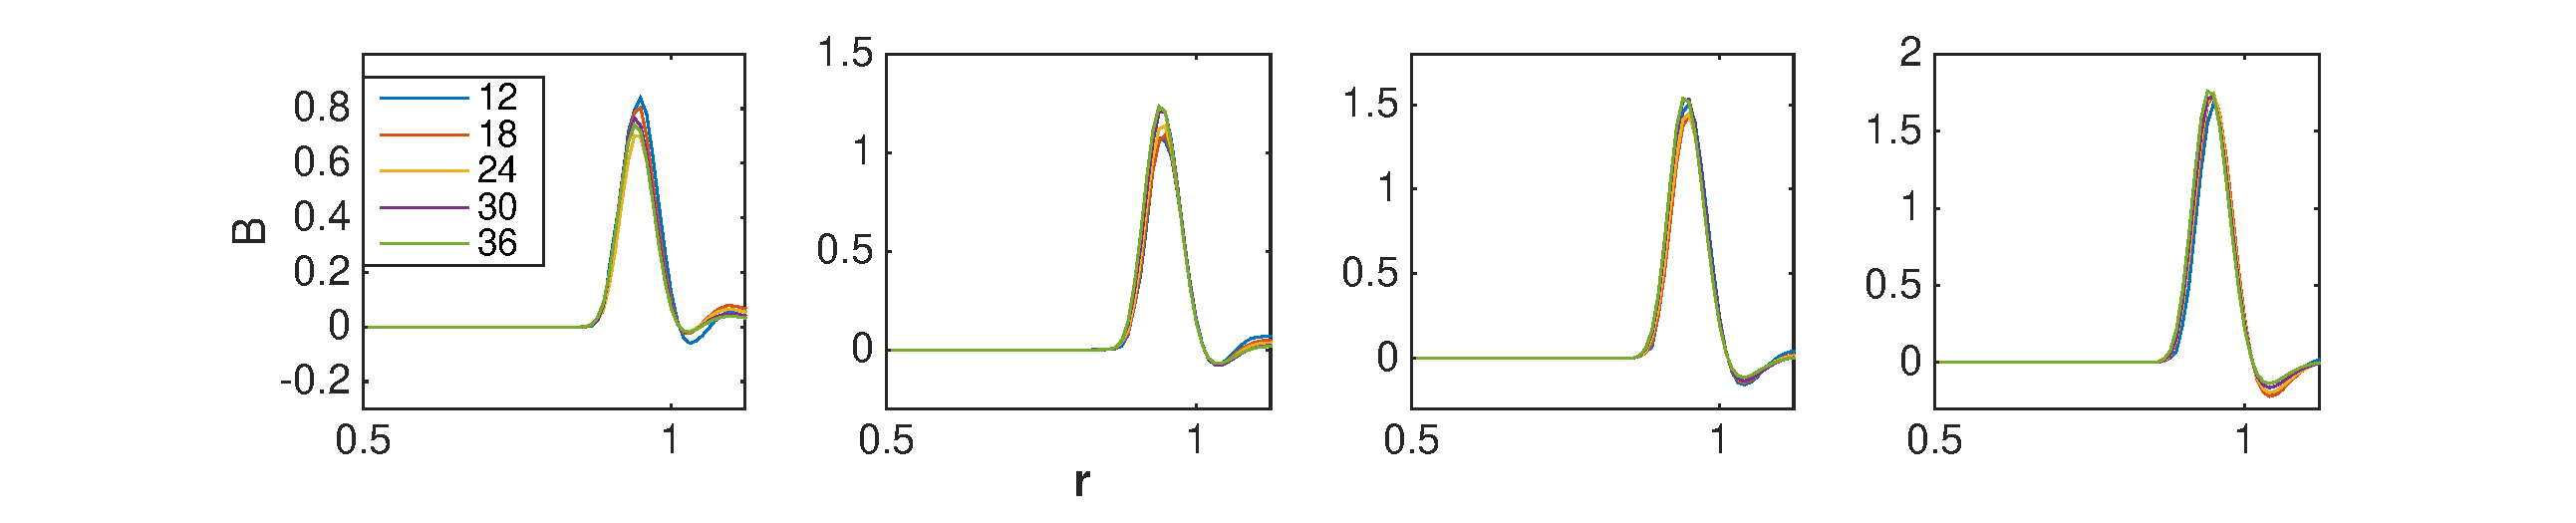
\includegraphics[width=1.0\linewidth]{del_u_sq-del_sq_u_overPesq.eps}
\caption{Plot of $B = \frac{\nabla u({\bf r})^2 - \nabla^2 u({\bf r}) d{\bf r}}{Pe^2}$ versus $Pe$. The four plots correspond to $\tau = 20, 30, 40, 50$ from left to right. }
\label{fig:B_versus_r}
\end{figure*}

We have explicitly included the $Pe$ scaling in the anisotropic component of the correlation function motivated by the $Pe^2$ scaling exhibited by the work. 
We now show that the relation $\langle {\bf F}^2 \rangle - \langle {\bf F}^2 \rangle_0$ can partially explain the observed renormalization of the isotropic pair-correlation function with the driving force $Pe$. 
%Assuming $|\nabla u({\bf r}) g({\bf r})$ is sharply peaked around $|{\bf r}|\approx \sigma$ given the rapid variation in the WCA potential, the integrals $\int \nabla^2 u({\bf r}) g({\bf r})$ and  $\int |\nabla u({\bf r})|^2 g({\bf r})$ can simply be expressed in the form $\int f(r) g_i({\bf r})\approx 2 \pi \sigma l f(\sigma) (g_{eq}(\sigma)+\Delta(\sigma)$. Here the length scale $l$ is set by width of the peak in the function $|\nabla u({\bf r}) g({\bf r})$. 

To proceed, we adapt Kirkwood's closure to approximate the three body correlation in terms of two body correlation functions. Specifically, we assume that $g_3({\bf r},{\bf r}^\prime)\approx c g_{eq}({\bf r} - {\bf r}^\prime) g({\bf r}) g({\bf r}^\prime)$ where $c$ is a normalization factor that satisfies $g_{3}({\bf {r} , \bf {r}'}) \approx c g_{eq}({\bf r} - {\bf r}^\prime) g_{eq}({\bf r})  g_{eq}({\bf r}') $ at equilibrium. % In this approximation the integral involving the three body correlation function simply reads 
%\begin{equation}
%\label{eq:simplify}
%\int  \int  \grad u({\bf r}) \cdot  \grad u({\bf r}')  g_3({\bf r}, {\bf r}') d{\bf r} d{\bf r}' = \langle F \rangle^2 +c \int \int \grad u({\bf r}) \cdot  \grad u({\bf r}') (g_{eq}({\bf r},{\bf r}^\prime)-1) g({\bf r}) g({\bf r}^\prime)
%\end{equation}
We now use the above-mentioned decomposition of $g({\bf r})$ into the equilibrium contribution and the isotropic and anisotropic corrections. We only keep terms up to order $\Delta ({\bf r})$ in the isotropic correction. We first note that the terms involving a single factor of the anisotropic contribution cancel to zero upon integration from symmetry considerations. The only terms that survive are terms quadratic in $\delta({\bf r})$ accompanied by a factor of $Pe^2$ and terms linear in $\Delta({\bf r})$:
\begin{equation}
\begin{split}
&\int (\nabla u(r)^2 - \nabla^2 u(r))  \Delta(r) d{\bf r}  = Pe^2 \alpha +\\ &Pe^2\left( \rho^2 \int \int \nabla u({\bf r}) \cdot \nabla u({\bf r}') g_{eq}({\bf r} - {\bf r}') \delta({\bf r}) \delta({\bf r}') d{\bf r} d{\bf r}' \right) .   \\
& +2 \rho^2  \int \int \nabla u({\bf r}) \cdot \nabla u({\bf r}') g_{eq}({\bf r} - {\bf r}') g_{eq}({\bf r}) \Delta ({\bf r}')  d{\bf r} d{\bf r}'
\end{split}
\label{eq:Kirkwood}
\end{equation}
where $\alpha = \dfrac{\langle {\bf F}^2 \rangle - \langle {\bf F}^2 \rangle_0}{Pe^2}\propto \langle \dot{w} \rangle/Pe^2$. Eq.~\ref{eq:Kirkwood} is an integral equation relation between $\Delta (r)$, $\delta({\bf r})$ and the rate at which work is performed $\langle \dot{w}\rangle$. Starting from the condition of energy balance, it constrains how the pair correlation function is modified due to non-equilibrium driving. 
%We note that Eq.~\ref{eq:Kirkwood} does not imply that $\Delta(r)$ simply scales with $Pe^2$ even though this is a valid solution. 


In Fig~\ref{fig:integral_A}, we plot estimates of $A \equiv \int (\nabla u(r)^2 - \nabla^2 u(r))  \Delta(r) d{\bf r}$ obtained from simulations, as a function of $Pe$ for various values of $\tau$. 
We find both a linear and an quadratic regime with the quadratic regime dominating in the high $Pe$ limit. The linear regime is not consistent with the scaling predicted in Eq.~\ref{eq:Kirkwood} and suggests a breakdown of the approximate closure relations, such as the Kirkwood approximation. In Fig~\ref{fig:B_versus_r} we show that the integrand itself is well approximated as a function of the form $Pe^2 f({\bf r})$ for the larger values of $Pe$ we explored. We note that one of the solutions permitted by Eq.~\ref{eq:Kirkwood} is that the isotropic renormalization of the pair correlation function simply scales like $Pe^2$. While this simple scaling is not observed in the simulations of the driven tracer-WCA particle system, Fig.~\ref{fig:integral_A} and Fig.~\ref{fig:B_versus_r} show how Eq.~\ref{eq:Kirkwood} can be used to anticipate weaker constraints on the renormalization of the pair correlation functions due to non-equilibrium driving. 

\section{Biasing the average work done on the tracer bath interactions can lead to a renormalization of interaction potentials}

As a final illustration of how work done on the tracer can modify the interactions in this system, we consider biasing the dynamics~\cite{Chetrite2013,Jack2010} with a function that on average would have equaled the work performed on the tracer in the driven liquid. For the theoretical calculations in this section, we explicitly represent the particles of the bath. We choose as our biasing function
\begin{equation}
\begin{split}
&h =\sum_{i \in bath} {\bf F}_i \nabla_i U_0 \\ &+\nabla^2_i U_0+{\bf F}_{0} \nabla_0 U_0 +\nabla^2_0 U_0  
\end{split}
\label{eq:biasingfunction}
\end{equation}
where $U_0$ is the energy of interactions between the tracer and the bath, ${\bf F}_i$ is the force on the $i^{th}$ bath particle, $i \neq 0$, ${\bf F}_0$ denotes the force on the tracer particle and ${\bf \nabla}_0$ denotes spatial derivatives with respect to the position of the tracer particle. For a tracer-bath system evolving according to Eq.~\ref{eq:xEOM} with $i=0$ denoting the tracer particle energy balance implies 
\begin{equation}
h+\dot{w} \equiv \left\langle \frac{d U_0}{dt}\right \rangle_{\eta}
\label{eq:defbias}
\end{equation}
where $\dot{w}=-{\bf F}. {\bf F}_d/\gamma$ and $\langle \dots\rangle_\eta$ is an average over the random noise terms. Instead of driving the system out or equilibrium using ${\bf F}_d\neq 0$, we consider Eq.~\ref{eq:xEOM} with ${\bf F}_d =0$ and sample trajectories biased by the exponential weighting function $\exp\left[-k H \right]$ where $H\equiv \int_0^{t_{obs}} h$ and $t_{obs}$ is the length of the trajectory.  Applying such a bias hence generates trajectories that preferentially cause energy flow into or extract energy from $U_0$. Sampling this ensemble of trajectories provides an indirect (if somewhat contrived) way to asses how energy flows can modify the properties of interacting many body systems. We note that such trajectory biases have been used in other contexts for instance to explore dynamical heterogeneities in glassy systems~\cite{Hedges2009}. 

As detailed in Ref~\cite{Chetrite2013}, physical dynamics with the same averaged properties as the biased dynamics detailed above can be constructed by solving the following eigenvalue equation 
\begin{equation}
\left[L^\dagger+k h\right]g(k)=\lambda(k) g(k)
\label{eq:adjointbiased}
\end{equation}
where $\lambda(k)$ is the cumulant generating function appropriate to the biasing field and $L$ is the Fokker-Planck operator evolving the probability distribution $p({\bf r}_i)$ of the tracer-bath system, $dp/dt = L p$. The force fields in the effective physical dynamics can be obtained by solving the eigenvalue problem in Eq.~\ref{eq:adjointbiased}~\cite{Chetrite2013}. Specifically averages computed using trajectories generated with force fields $\tilde {\bf F}_i \equiv {\bf F}_i + \nabla_i \ln g(k)$ will match averages extracted from the biased dynamics~\cite{Chetrite2013}. Usually, such effective force fields $\tilde {\bf F}_i$ are highly non-trivial and are tough to compute. 

We find that simple intuitive expressions for the effective force fields can be derived by solving Eq.~\ref{eq:adjointbiased} perturbatively. Specifically, we expand $g(k)=g_0 + k g_1 + \dots$ and $\lambda(k)= \lambda_0 + k \lambda_1+ \dots$. Here, $g_0(r)\propto 1$ is the uniform left eigenvector of $L$ and $\lambda_0=0$. Using this perturbation expansion and collecting terms with similar powers of $k$, we see that $\lambda_1= \langle g_0 | h |u_0\rangle$ where $u_0$ is the steady state of $L$, $L |u_0\rangle=0$. Since, we imagine applying the biasing fields to undriven tracer bath systems, no energy is exchanged at equilibrium and $\lambda_1=0$. The first order correction $g_1$ hence satisfies 
\begin{equation}
L^\dagger g_1 = -h
\label{eq:solution}
\end{equation}
The action of the adjoint operator is given by 
\begin{equation}
\begin{split}
& L^\dagger g_1  =\sum_{i \in bath} {\bf F}_i \nabla_i g_1 +\nabla^2_i g_1 \\& +{\bf F}_{0}\nabla_0 g_1 +\nabla^2_0 g_1 =h 
\end{split}
\label{eq:adjoint}
\end{equation}
From Eq.~\ref{eq:adjoint} and Eq.~\ref{eq:biasingfunction} it is clear that Eq.~\ref{eq:solution} is solved by $g_1=-U_0$. Hence, the force between the tracer and the bath in the effective dynamics mimicking the biased ensemble, $\tilde {\bf F}$ is simply equal to 
\begin{equation}
\begin{split}
\tilde {\bf F} &= {\bf F} + {\bf \nabla} \ln \left[1-k U_0\right] \\
& ={\bf F} - k{\bf \nabla} U_0
\end{split}
\label{eq:effectivedynamics}
\end{equation}
In other words, biasing fields that generate trajectories that consume energy from or release energy into the tracer bond potential $U_0$ are mimicked by physical dynamics in which the tracer-bath interactions are modified. The bath-bath interactions and tracer-tracer interactions remain unmodified in the effective dynamics. By tuning the energy consumption rates through $k$ in the biased ensemble, the structural properties of the liquid can effectively be modified as described by Eq.~\ref{eq:effectivedynamics}. 
While this analysis is perturbative, it provides intuition for the interplay between energy consumption and structural reorganization. Indeed, in the limit that the imbalance between the tracer-bath and bath-bath/tracer-tracer forces due to the biasing in Eq.~\ref{eq:effectivedynamics} reaches $k_BT/\sigma$, where $\sigma$ is the particle size, tracer-bath phase separation can be achieved. 
\section{Conclusions}
Developing techniques to characterize and control the behavior of far-from- equilibrium systems remains a central and outstanding problem in non-equilibrium thermodynamics. In this paper, we have shown that in certain limits, specifying simple scalar observables such as $\langle w \rangle$ or energy consumption rates allows us to constrain the transport and structural properties of our far-from-equilibrium system. It remains to be seen if similar results can be obtained in other more complex systems with anisotropic building blocks such as active liquid crystals or driven chiral objects~\cite{Joshi2017,vanZuiden2016,Nguyen2014b}. Such extensions will be pursued in future work.  

\bibliography{DrivenDisks_v6.bib}

\end{document}
\section{Pair Correlation Function As Predicted by Theoretical Model  --- Optional stuff}

Note to Suri:  I was not sure you wanted to include this at all in the paper, so I just moved this to the end.



As far as the pair correlation function of the tracer is concerned, we can easily access its form by noting that $\langle {\bf F}^2 \rangle_0 $ can be expressed as:

\begin{align}
\langle {\bf F}^2 \rangle_0 & =  K_B T  \rho \int  \grad^2 h u({\bf r})  g({\bf r}) d{\bf r}\\
& = K_B T  \rho \int  |{\bf q}|^2 h V({\bf q})  g({\bf q}) d{\bf q}
\label{eq:fsqzerofinal}
\end{align}

Comparing Eq. \ref{eq:fsqzerofinal} to Eq. 41 in the SI, we get that:

\begin{equation}
\langle {\bf F}^2 \rangle_0 = \dfrac{h^2}{\gamma^2} \int d{\bf q} \dfrac{|V({\bf q})|^2}{K({\bf q})} \left( 1 - \dfrac{Pe^2 |{\bf v}|^2}{ [\frac{K_BT}{\gamma_G} K({\bf q}) + D_0 ]^2} \right) 
\label{eq:FSqZero}
\end{equation}

\begin{equation}
g({\bf q}) = g_{eq}({\bf q}) - \dfrac{h}{\gamma^2 K_B T} \dfrac{Pe^2 {\bf v}^2}{ \left[ \frac{K_B T}{\gamma_G} K({\bf q}) + D_0 \right]^2 }
\label{eq:FSqZero}
\end{equation}




Note to Suri:  I am again not sure these next two pictures still belong in the paper, since we are focusing on that integral.


\begin{figure}[!ht]
\centering
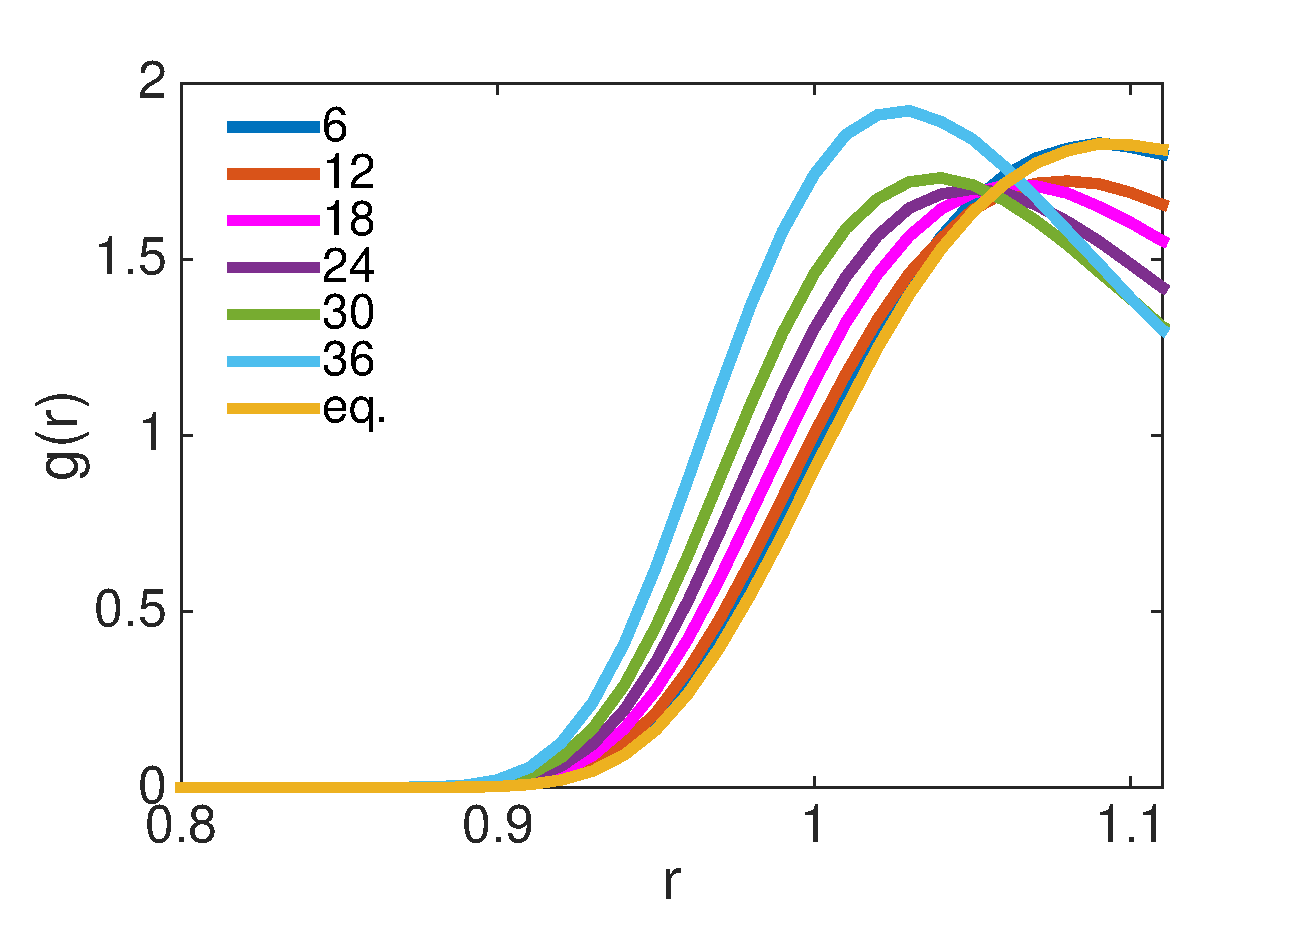
\includegraphics[width=0.5\linewidth]{gr_vs_r_tau_20.eps}
\caption{Plot of the pair correlation function for a system with tau=20 and at various values of Pe. The sampled values of Pe were 6, 12, 18, 24, 30 and 36. The pair correlation function g(r) was computed as the average probability of finding an inactive particle at a distance between r and r+dr of an active particle, in a simulation with 10\% active particles. The x axis is cut off at $\sigma=1.12$, the cutoff parameter used with the WCA potential.}
\label{fig:gr_vs_r}
\end{figure}


\begin{figure}[!ht]
\centering
\includegraphics[width=0.55\linewidth]{gr_vs_r_tau_20_div_Pe_sq.eps}
\caption{Plot of the pair correlation function in Fig. \ref{fig:gr_vs_r} scaled by $Pe^2$. We only show values of $Pe$ > 6 because as in the case of the diffusion constant, it is only at medium - large values of $Pe$ that the $Pe^2$ scaling becomes the dominant contribution.}
\label{fig:gr_div_pe_sq}
\end{figure}



